%\chapter{Background/History of the Study }


\section{Background}

In their paper Vinyals et al (2015)\cite{DBLP:journals/corr/VinyalsL15} discuss making a chatbot using
a neural network configured for sequence to sequence neural machine
translation. We code our own sequence to sequence chatbot, though our results are less than
spectacular. As our hand coded model does not run sufficiently well, we use code authored by Matthew Inkawhich (2018)\cite{2018Inkawhich}.

In their paper Vaswani et al (2017)\cite{Vaswani2017AttentionIA} discuss using the Transformer architecture for solving machine learning tasks. We train a transformer model as a chatbot.


Also Radford et al (2019)\cite{radford2019language} discuss the GPT2 neural network for NLP tasks. The GPT2 model is based largely on the Transformer architecture. GPT2 stands for 'Generative Pre-training Transformer 2'. 

We implement a chatbot with a GPT2 model. We use a program library from Wolf et al (2019)\cite{Wolf2019HuggingFacesTS} to run our model.


It is worth noting that with the appearance of the Transformer architecture and WordPiece vocabulary scheme, some technologies have become redundant or obsolete. This may be true of any model that uses RNN components and also the traditional word vector embeddings.

\section{Recursive Neural Network Components}

The goal behind RNN components is to detect patterns. Here we explore a simple RNN.

The simplest RNN has two inputs and two outputs. They can be arranged in chains. In our example the input will be a sequence of data and the RNN chain will be a line of components of the same length.

One input from each component is the hidden state output from the RNN to the left. Another input is the current input from the sequence that the chain is monitoring. One output is the generated hidden state, meant for the component to the right. The last output is the value that the RNN surmises. 

In our diagram the two inputs are labeled on the left side, and the single output does double duty as both the hidden state output and the value that the RNN surmises.

There are several designs for an RNN component. The inner workings of these components are what makes them different. In the example in the diagram the inner workings are very simple. Two paths, labeled as inputs, take data into the RNN. Their data is combined in the green circle. This combination is done with concatination and simple feed forward neural network components. The output from the concatination is passed through the red circle. This is a tanh activation operation that limits the output to values from -1 through 1. This tanh activation keeps the output within reasonable values. Finally the output is delivered outside the component to the program employing the RNN. In this diagram there is only one output. The single output would serve as both the hidden state output for that position in the chain, and also the data output component for that position in the chain.

\begin{figure}[H]
	
	\includegraphics[scale=0.5]{diagram-rnn}
	
	RNN - 1 and 2 are inputs, 3 is the output.
	
	\addcontentsline{lof}{section}{Recurrent Neural Network}
\end{figure}

A second type of RNN is the GRU. GRU stands for 'Gated Recurrent Unit'. A GRU has two inputs and two outputs. The formulas for a GRU, as outlined by Denny Britz in the website WILDML (Britz 2015)\cite{2015Britz}, are as follows.


$$ z =\sigma(x_tU^z + s_{t-1} W^z) $$  
$$ r =\sigma(x_t U^r +s_{t-1} W^r) $$  
$$ h = tanh(x_t U^h + (s_{t-1} \circ r) W^h) $$  
$$ s_t = (1 - z) \circ h + z \circ s_{t-1} $$  


The GRU has two inputs and two outputs. It also has two internal gates. One internal gate is the 'reset' gate. This one determines how much of the previous input is combined with the new value calculated by the mechanism of the GRU. It is denoted as '$r$' above. Another internal gate is the 'update' gate. The update gate decides how much new information is to be included in gate computation. It is denoted as '$z$'.

Here '$ s_t $' is the symbol for the output. '$h$' is the symbol for the 'hidden output'. The two inputs are '$ x_t $' and '$ s_{t-1} $' . '$ x_t $' is the hidden state input. '$ s_{t-1} $' is the regular input for the RNN or GRU. Sigmoid activation is used on the two gates, while tanh activation is used to compute the hidden output.

In the last line, the regular output is determined using the 'dot' product which is denoted with a circle, along with an addition operation. In the two gate formulas (the first and second) the output is determined as the sum of two matrix multiplication operations passed through sigmoid activation. This produces values in the range of 0 to 1.

Under most programming circumstances the GRU is not implemented by the average programmer. The programmer employs a language like python and a programming library like Pytorch or Tensorflow. The library then implements the GRU and makes it easy for the programmer to use that implementation.

\section{Sequence to Sequence}

Translating text from one language to another has become a common task for computers. The Sequence to Sequence architecture is often used today  for this purpose.

A naive approach to translation involves using a dictionary. You would encode each key as a word from one language and the value for that key would be the translated word in the target language. Of course this doesn't work, because different languages not only have different words for the same thing, but they also have different sentence structures for what might be similar concepts.

A better approach is sequence to sequence translation. A description follows with a section at the end for how training works.

In this approach we use recurrent neural networks to obtain our translation. Two recurrent neural network components are employed. One is responsible for the input language and the other for the output. Recurrent elements can remember sequences. 

Also employed are two vocabulary sets. One vocabulary is for the source language and another is for the target language. A table of word vectors the size of the input vocabulary is created and a maximum sentence length is picked. There is also a 'hidden size', which is an important dimension in the model. In practice the hidden size could be between 300 and 550 for this kind of application.

First text is prepared for training. A text corpus with source and target pairs is chosen. Sentences in the source corpus are paired with sentences with the same meaning in the target corpus. Sentence length is observed and for all shorter sentences a special 'end-of-sequence' token is appended to all sentences in both languages.

Word vectors are created composed of floating point numbers. Each word in the vocabulary is translated to an integer which remains the same throughout the use of the translator. The word vectors are arranged in a table of floating point numbers with one dimension being the size of the input vocabulary and one dimension being the hidden size for the vector.

The recurrent unit in this case is a GRU. This stands for Gated Recurrent Unit. The GRU takes as input a single vector. It processes the vector and returns another vector. This could be
exactly the same as the input or somehow changed. The input vector and the output vector have the
dimension of the 'hidden size' mentioned above. Throughout the discussion of this model the hidden size will remain the same.

So far the model takes a word, translates it to an integer, and finds the vector in the word embedding table that represents that word. Then it gives the entire vector to the GRU. The GRU takes the word and decides weather to return as output just the input or the input modified.

The input segments composed of GRUs take two input vectors and return two output vectors. Later we will use GRUs to construct output segments. Here we want to stress that the inputs cascade from GRU to GRU in the input segment. 

The first word in the input sentence is converted to a vector and passed to the first GRU. The GRU has two inputs and two outputs. One input is for new data and one is for the hidden state of the segment in question. The first GRU consumes the first word. The second GRU takes the hidden state from the first GRU along with the second word and consumes them.

The third GRU takes the hidden output from the second GRU and the third word and consumes them. This pattern is repeated for the length of the input sentence. A complicating detail is that although many GRUs are called for in the input segment they all use the same set of weights and 
biases. For this reason only a single input GRU is used for all of the words in practice. Outputs are calculated and then cycled around and fed with the next word from the sentence in vector form to the input of the GRU. 

One at a time all the words from the input sentence are passed to the input GRU. The hidden state
from the last GRU is passed to the output segment. The output segment is also GRU based.

The output is in charge of generating tokens that represent the input in the output language. The output uses GRU segments also. The first hidden input for the first output is taken from the 
last hidden output of the last recursive unit of the input chain. It is important because it is the spot where a great amount of data is passed from the input section to the output section. 
The connection at this point is said to carry the 'thought vector'. Most of the information responsible for translating one language to another is passed at this point.

The hidden values from the input section are passed to the first output GRU. It outputs the values that are converted to the first word of the output. The first output GRU also has a hidden state. It passes the first word and the hidden state on to the second GRU.

The second GRU generates the second word and also its own hidden state. The second word is recorded and the word and the hidden state are passed on the the next GRU. This is repeated until a special 'end-of-sequence' token is found or until the number of tokens equals the maximum number allowed.

\begin{figure}[H]
	
	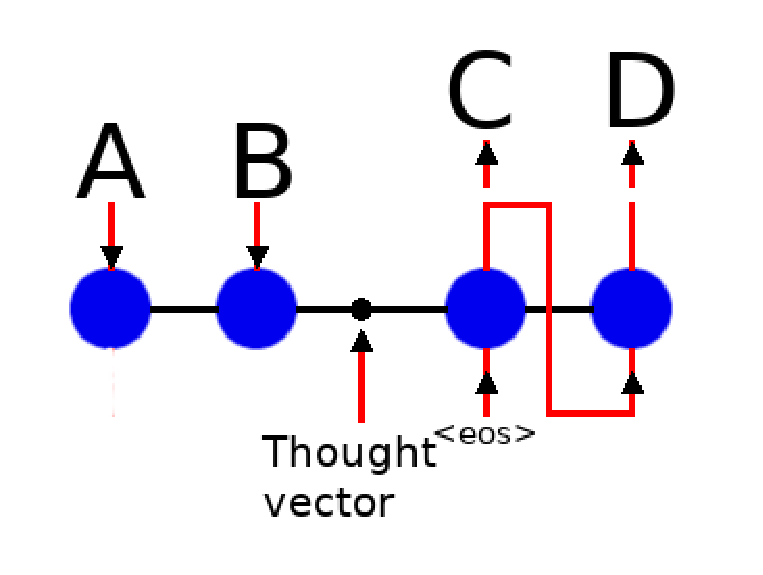
\includegraphics[scale=0.5]{diagram-nmt}
	
	Seq2seq: A and B represent an input sequence and C and D represent
	the corresponding output.
	
	\addcontentsline{lof}{section}{Sequnce to Sequnce}
\end{figure}

Each output we have is currently in the form of a vector. These vectors are a long string of floating point numbers, each one the dimensions of the 'hidden size' mentioned above. What's done with them is they are converted to the dimensions of the output vocabulary. Then they are processed in what is called an 'arg-max' function. This processing determines the index of the maximum value in the new vocabulary sized vector. This index allows the program to look up the corresponding word in the output vocabulary. This word is then used as the model output at that point in the output chain.

How does the model know what target vocabulary indexes go at what point in the output? For this we refer back to the corpus that we already have. One part of the corpus is the source language. The other part is the target language. A sentence is applied to the input and for that sentence an output is generated. The output is called a prediction. If the target and the prediction are not the same, the model must modify itself so that in the future they are.

That ends our discussion of Sequence to Sequence Translation. This is how some computer models do language translation. 

There are some inherent problems. Because the output of a GRU is constantly being reused as the input, lots of data that might be useful to have is lost when the GRU churns through internal operations where several matrix multiplication operations are performed together on input. With every iteration more data is lost and so, for example, the effective length of the input and output sentences must be short. 

Another problem is that all input to be translated to target output has to be boiled down and 
passed to the output section through a small corridor the size of a typical word vector. This channel is sometimes referred to as the 'thought vector.' Somehow all necessary information must be there. This also limits the length of the input and output vectors. It does help, when setting
up a model for later training, to make the hidden size larger, but it only helps so much. There is a point at which the benefit of increasing the hidden size is lost.

\section{Loss and Accuracy}

At first the prediction from a model is not very close to the desired output. The output is compared to the prediction and a 'loss' is generated. 'Loss' measures the difference between the predicted output and the target. A larger loss represents two values, prediction and target, that are further apart. The loss function must be chosen. 

%A typical loss function is 'Mean Squared Error' or MSE.

Another metric is Accuracy. 'Accuracy' is a numerical representation of the difference between the desired output and the generated prediction. It is a percentage of the time that the output is exactly correct.

Getting a prediction, running input data through a neural network, is forward propagation.
Training, then, is a mathematical process involving backpropagagtion. Backpropagation identifies areas of the model that need to be modified in order to get the proper prediction in the future.

%\iffalse
In practice we take the derivative of the loss function in order to backpropagate. The derivative is multiplied by the learning rate and subtracted from the original weight value. The result is a set of adjusted weight matrices. When these matrices are used later they allow for better predictions. 
%\fi

This is done over and over with every source/target sentence pair. Slowly the model is changed and predictions start to match the target. That's training. The loss should decrease over time and the accuracy should increase.

There are several numerical metrics that we can record during training that tell us how our model is training. The loss, a mathematical calculation of the difference between the model's output and the predicted value, is mentioned above. Loss is an important number. Also accuracy is important. Accuracy is a mathematical calculation of the difference between the model's output and the value that output should be, but it focuses on the number of times the model comes out with a correct prediction verses how many output values there are in total.

\section{Attention Mechanism}

\section{Sequence to Sequence Chatbot}
